%start preamble
\documentclass[paper=a4,fontsize=11pt]{scrartcl}%kind of doc, font size, paper size
\usepackage[ngerman]{babel}%for special german letters etc			
%\usepackage{t1enc} obsolete, but some day we go back in time and could use this again
\usepackage[T1]{fontenc}%same as t1enc but better						
\usepackage[utf8]{inputenc}%utf-8 encoding, other systems could use others encoding
%\usepackage[latin9]{inputenc}			
\usepackage{amsmath}%get math done
\usepackage{amsthm}%get theorems and proofs done
\usepackage{graphicx}%get pictures & graphics done
\graphicspath{{pictures/}}%folder to stash all kind of pictures etc
\usepackage{amssymb}%symbolics for math
\usepackage{amsfonts}%extra fonts
\usepackage []{natbib}%citation style
\usepackage{caption}%captions under everything
\usepackage{listings}
\usepackage[titletoc]{appendix}
\numberwithin{equation}{section} 
\usepackage[printonlyused,withpage]{acronym}%how to handle acronyms
\usepackage{float}%for garphics and how to let them floating around in the doc
\usepackage{cclicenses}%license!
\usepackage{xcolor}%nicer colors, here used for links
\usepackage{wrapfig}%making graphics floated by text and not done by minipage
\usepackage{dsfont}
\usepackage{stmaryrd}
\usepackage{geometry}
\usepackage{hyperref}
\usepackage{fancyhdr}
\usepackage{menukeys}

%settings colors for links
\hypersetup{
    colorlinks,
    linkcolor={blue!50!black},
    citecolor={blue},
    urlcolor={blue!80!black}
}

\definecolor{pblue}{rgb}{0.13,0.13,1}
\definecolor{pgreen}{rgb}{0,0.5,0}
\definecolor{pred}{rgb}{0.9,0,0}
\definecolor{pgrey}{rgb}{0.46,0.45,0.48}

\pagestyle{fancy}
\lhead{Netzwerke Übung (SoSe 2019)}
\rhead{FB 4 -- Angewandte Informatik\\ HTW-Berlin}
\lfoot{Übungsblatt 03 -- Routing}
\cfoot{}
\fancyfoot[R]{\thepage}
\renewcommand{\headrulewidth}{0.4pt}
\renewcommand{\footrulewidth}{0.4pt}

\lstdefinestyle{Bash}{
  language=bash,
  showstringspaces=false,
  basicstyle=\small\sffamily,
  numbers=left,
  numberstyle=\tiny,
  numbersep=5pt,
  frame=trlb,
  columns=fullflexible,
  backgroundcolor=\color{gray!20},
  linewidth=0.9\linewidth,
  %xleftmargin=0.5\linewidth
}

\newlength\labelwd
\settowidth\labelwd{\bfseries viii.)}
\usepackage{tasks}
\settasks{counter-format =tsk[a].), label-format=\bfseries, label-offset=3em, label-align=right, label-width
=\labelwd, before-skip =\smallskipamount, after-item-skip=0pt}
\usepackage[inline]{enumitem}
\setlist[enumerate]{% (
labelindent = 0pt, leftmargin=*, itemsep=12pt, label={\textbf{\arabic*.)}}}

\pdfpkresolution=2400%higher resolution

%%here begins the actual document%%
\newcommand{\horrule}[1]{\rule{\linewidth}{#1}} % Create horizontal rule command with 1 argument of height

\DeclareMathOperator{\id}{id}

\begin{document}
\begin{center}
\Large{\textbf{Hausaufgaben -- Routing}}\\
\end{center}
Nachdem Sie in der letzten Übung einige Grundlagen im Bereich Linux und Netzwerktechnik kennengelernt haben, soll im Folgenden darauf aufbauend Ihr Wissen erweitert werden. Mit diesem Hausaufgabenblatt sollen die Fundamente für die Umsetzung eines einfachen, statisch gerouteten Netzwerks gelegt werden.\\
Inhalt:
\begin{itemize}
	\item Grundlagen Routing, Routing-Protokolle \& Einordnung ins OSI-Modell 
	\item CIDR-Notation
	\item Planung eines Netzwerkes mitsamt Linux-Router
	\item Erweiterung der Tools für Netzwerkadministration
	\item Routing im Kernel
\end{itemize}
Hilfreiche Links:
\begin{itemize}
	\item \url{https://en.wikipedia.org/wiki/Routing}
	\item \url{https://en.wikipedia.org/wiki/Classless_Inter-Domain_Routing}
	\item \url{http://linux-ip.net/html/part-reference.html}
	\item \url{ http://linux-ip.net/html/tools-ip-management.html}
	\item \url{https://wiki.debian.org/NetworkConfiguration#Multiple_IP_addresses_on_one_Interface}
	\item \url{http://linux-ip.net/html/tools-route.html}
	\item \url{https://www.techrepublic.com/article/understand-the-basics-of-linux-routing/}
\end{itemize}

\begin{center}
\Large{\textbf{Aufgabe A -- Routing Grundlagen}}
\end{center}
\vskip0.25in
Nachdem Sie im letzten Übungsblatt Ihr Netzwerk durch einen Switch verbunden haben und hierdurch Ihre Kommunikation aufgebauten, \glqq wandern\grqq\ Sie im kommenden Übungsblatt im OSI-Modell eine Schicht weiter nach oben. Es soll folglich ein Netzwerk geplant sowie umgesetzt werden, das auf Routing setzt -- der Router ist fortan zentrale Anlaufstelle für die Kommunikation! Diese Umsetzung hat den Vorteil, dass der Router Pakete über Netzgrenzen hinweg vermitteln kann. Ihr kleines, abgeschottetes Netzwerk kann über die bisherigen Grenzen hinweg kommunizieren.
\begin{enumerate}
	\item Lesen Sie folgenden Artikel: \url{https://en.wikipedia.org/wiki/Routing}
	\item Was sind die Aufgaben eines Routers. Wie erfolgt, im Groben, die Umsetzung des Routings?
	\item Routing kann unterschiedlich kategorisiert werden, nennen Sie die Kategorien und deren Bedeutung.
	\item Nennen Sie einige Routing-Protokolle. Ist Ihnen eines (oder mehrere) dieser Protokolle bereits begegnet?
	\item Machen Sie sich klar, wie Router und IP-Protokoll zusammenhängen.
	\item In welche Schicht des OSI-Modells würden Sie einen Router einordnen? (Begründung!)
	\item Wie haben sich bis jetzt Ihre Raspberry Pis gefunden? Woher \glqq wussten\grqq\ sie, an welches Gerät die Ethernet-Frames zu schicken waren? Wie spielt hier Ihre eigene IP-Adresse, Ihre Subnetzmaske mit hinein? Bzw. spielt diese auf Hardwareebene eine Rolle?
	\item Woher weiß ein Rechner, wann er ein Paket direkt adressieren kann und wann er es an Router/Gateway weiterschicken muss?
	\item Woher weiß ein Router, wann er ein Paket weiterschicken soll und wann nicht?
\end{enumerate}

\begin{center}
\Large{\textbf{Aufgabe B -- Planung des Routing zwischen Netzen}}
\end{center}
\vskip0.25in
Im vorigen Aufgabenblatt haben Sie zu den IP-Adressen auch eine Netzwerkmaske konfiguriert. Diese Netzwerkmaske legt fest, welche Rechner im gleichen (Sub-)Netz liegen und somit direkt angesprochen werden können. Daraus folgt aber auch, dass bestimmte Rechner außerhalb Ihres Netzes nicht direkt angesprochen werden können. Diese können via Router/Gateway erreicht werden.\\
Wir wollen in einem ersten Schritt selber einen Router betreiben, um über unsere kleinen Netze hinweg zu kommunizieren. Dazu erweitern Sie Ihr Wissen aus dem vorigen Übungsblatt, sodass Ihr Netzwerk im Labor \glqq wachsen\grqq\ kann.
\begin{enumerate}
	\item Früher wurden Klassen von Adressen genutzt, heute das \emph{CIDR (Classles Inter Domain Routing)}. Worin unterscheiden sich \emph{CIDR} und klassenbasierten Adressen?
	\item Recherchieren Sie, warum sich dies änderte!
	\item Recherchieren Sie wie die Syntax der klassenbasierten Notation aussieht und geben Sie einige Beispiele für die Notation.
	\item Recherchieren Sie wie die Syntax der \emph{CIDR}-Notation aussieht und geben Sie einige Beispiele für die Notation.
	\item Wie in der letzten Übung arbeiten Sie in Gruppen von je vier Studierenden.\\
	Um zwischen den beiden lokalen Netzwerken kommunizieren zu können, benötigen Sie einen Router. Einer der Raspberry Pis  soll diese Aufgabe übernehmen. \footnote{Wenn genug Raspberry Pis vorhanden sind, kann auch ein extra Raspberry die Rolle des Routers übernehmen} Die Rechner müssen so konfiguriert werden, dass sie wissen wohin die Pakete geschickt werden -- das heißt: Pakete die nicht in das eigene lokale Netzwerk gehören werden über den Router in die externen Netzwerke weitergereicht.
	\begin{figure}[H]
	\centering
	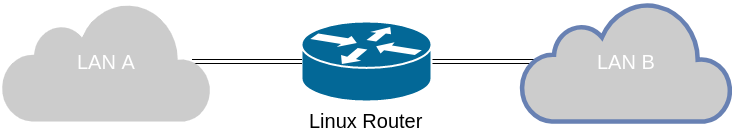
\includegraphics[scale=0.35]{lan}
	\caption{Skizze des Netzwerkes bestehend aus zwei LANs und einem Linux-Router}
	\end{figure}
	\begin{tasks}
		\task~ Unterteilen Sie Ihre Gruppe, sodass sich im Idealfall zwei Raspberry Pis in einen lokalen Netzwerk A und zwei Raspberry Pis im lokalen Netzwerk B befinden.
		\task~ Skizzieren Sie Ihre lokalen Netzwerke, sowie das gesamte Netzwerk (D.h. nutzen Sie geeignete Symbole s. letztes Übungsblatt).
		\task~ Vergeben Sie entsprechende IP-Adressen und kleinst mögliche Subnetzmasken auf der Skizze. Wählen Sie ein ähnliches Adressschema, wie in der letzten Laborübung.
		\task~ Planen Sie ebenso den Router mit entsprechenden IP-Adressen auf der Skizze ein. Achten Sie darauf, dass der Router als Verbindungsstück (Intermediate-Node/ Zwischenknoten) zwischen Ihren beiden Netzen fungiert und dementsprechend beide Netzwerke kennen muss. Das heißt, der Router muss zwei IP-Adressen haben, jeweils eine pro Netzwerk.
	\end{tasks}
\end{enumerate}

\begin{center}\Large{\textbf{Aufgabe C -- Planung des Backbones}}\end{center}\vskip0.25in
Aufbauend auf den kleinen LANs pro Tischreihe, soll eine größere Netzwerkinfrastruktur aufgebaut werden -- ein sogenanntes Backbone. Die kleinen Separaten Netzwerke werden verknüpft, darüber hinaus sollen Sie für einen Anschluss an das Internet sorgen (der sogenannte Uplink). Wie oben erwähnt wird im wesentlich ein solches Netzwerk als Backbone-Netzwerk beschrieben. Backbone-Routing wird auch an den großen Internet-Knoten umgesetzt (diese werden als Internet-Exchange-Point -- IXP bezeichnet), wie etwas dem \emph{DECIX} (\url{https://www.de-cix.net/}).
Im wesentlichen erweitern Sie den Aufbau Ihres Netzwerkes -- jedes LAN bekommt lediglich einen extra (Backbone) Router. Das Netzwerk soll im wesentlichen dem in Abb. \ref{backbone} entsprechen.
	\begin{figure}[H]
	\centering
	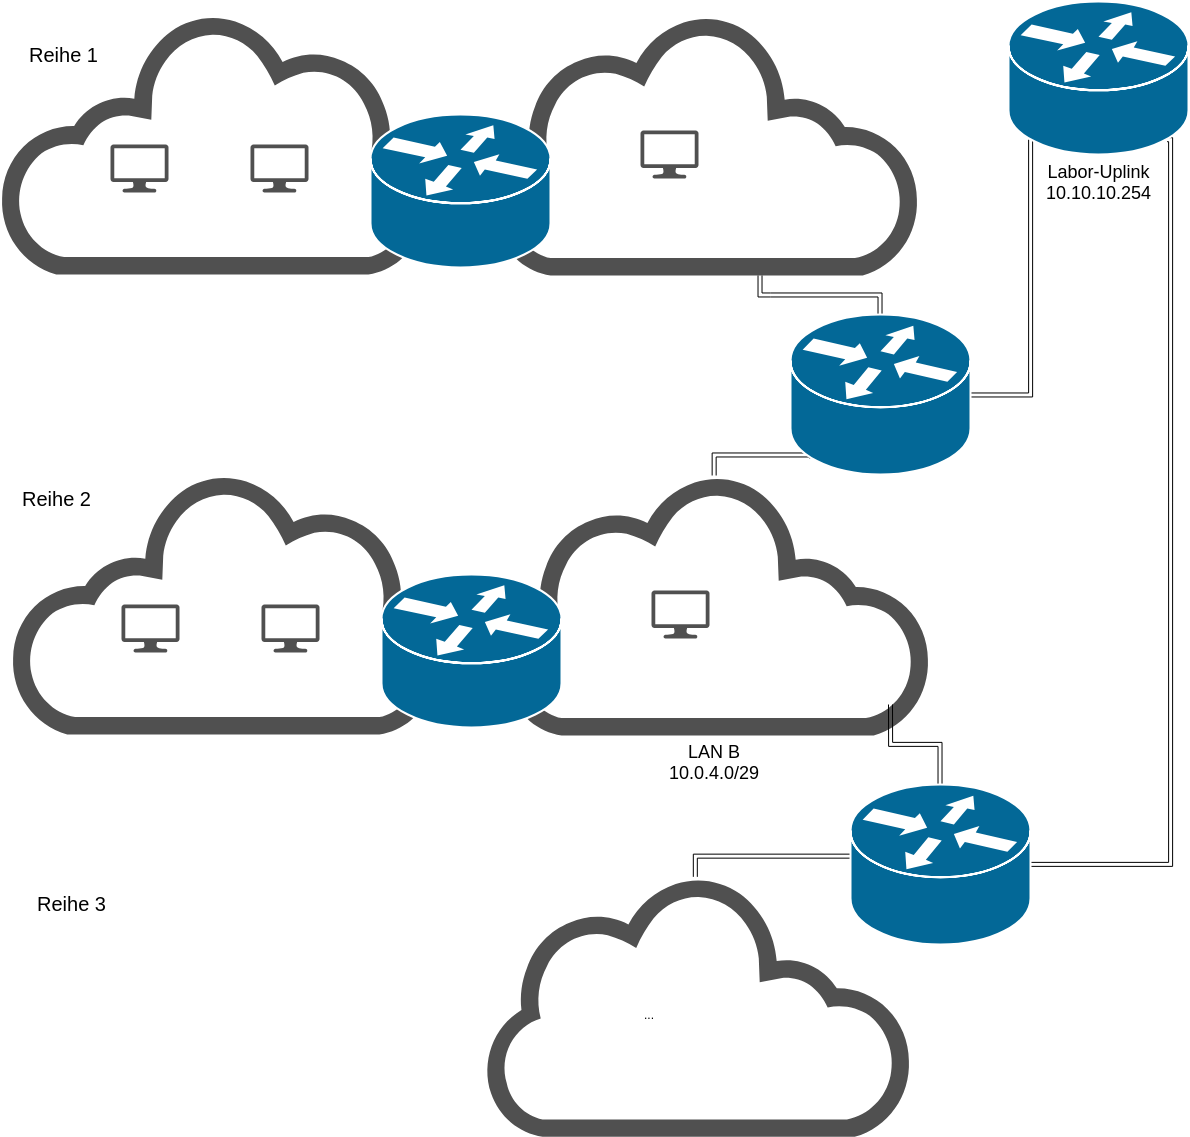
\includegraphics[scale=0.25]{backbone}
	\caption{Skizze des Netzwerkes bestehend aus fünf Bankreihen á zwei LANs, sowie den Backbone-Routern}
	\label{backbone}
	\end{figure}
Folgendes Adressschema gilt:
\begin{table}[H]
\caption{Adressschema für das Labor}
\label{adress_scheme}
\centering
\begin{tabular}{|c|c|}\hline
 & \textbf{IP  || IP-Range} \\ \hline
 $LAN_X$ & 10.0.$X$.Y/Size \\ \hline
 Backbone & 10.10.10.100 + $\rho$ \\ \hline
 Labornetz & 10.0.0.0/8 \\ \hline
 Uplink & 10.10.10.254 \\ \hline
 DNS & 10.10.10.254 \\ \hline
\end{tabular}
\end{table} 
$LAN_X$ bezeichnet die beiden Netzwerke (Ihre Bankreihe mit je zwei Subnetzen), wobei der Wert $X$ der Reihe nach hochgezählt wird. D.h. Bankreihe eins: $LAN_{1}$, Bankreihe zwei: $LAN_{2}$ etc. Beachten Sie hierbei, dass Sie festlegen müssen wo ein Netzsegment beginnt und wo dies auch endet. 
\begin{tasks}
		\task~ Planen Sie entsprechend der Skizze Ihr Netzwerk. D.h. planen Sie entsprechende IP-Adressen, Subnetzmasken und Router ein.
		\task~ Skizzieren Sie Ihre lokalen Netzwerke, sowie das gesamte Netzwerk mitsamt der Router (Nutzen Sie geeignete Symbole).
		\task~ Planen Sie ebenso den Backbone-Router, sowie den Uplink (Router im Rack -- Zugang zum DFN(Internet) ein.
	\end{tasks}

\begin{center}
\Large{\textbf{Aufgabe D -- Tools \& OS}}
\end{center}
\vskip0.25in

\begin{enumerate}
	\item Seit der letzten Übung kennen Sie schon einige grundlegende Befehle, um das Netzwerkinterface eines unixoiden Betriebssystems zu konfigurieren. Dieses Wissen soll nun erweitert werden. Hierfür schauen wir in die bekannten Werkzeugkästen \emph{iproute2} und \emph{net-tools}.
	\begin{tasks}(1)
	\task~ Recherchieren Sie, welches Tool des \emph{iproute2} genutzt werden kann um Routen zu setzen. Notieren Sie sich die Syntax und was die Parameter bewerkstelligen.
	\task~ Analog dazu: Wie werden Routen mithilfe der \emph{net-tools} konfiguriert?
	\task~ Recherchieren Sie beispielhaft wie eine persistente Lösung aussähe. Kommentieren Sie Ihr Beispiel anschließend, sodass Sie wissen was die einzelnen Zeilen bedeuten.
	\end{tasks}
	\item Gateways \& Router -- Gateways sind im allgemeinen nicht das Gleiche wie Router. Auch unter den Gateways gibt es Unterscheidungen.
	\begin{tasks}(1)
	\task~ Recherchieren Sie worin sich Router und Gateways unterscheiden.
	\task~ Beim aufsetzen des Netzwerkes kann unterschieden werden zwischen \emph{Gateways} und \emph{Default Gateways}. Recherchieren Sie diese Unterscheidung. Erläutern Sie die Ursache des Unterschieds.
	\end{tasks}
	\item Im vorigen Übungsblatt arbeitete Ihr Netzwerk mithilfe eines Switches. Alle Knoten des Netzwerkes waren innerhalb eines Segments (LAN). Daher konnte Sie nur innerhalb Ihres Netzwerkes kommunizieren, darüber hinaus aber nicht. Mithilfe eines Routers erweitern Sie die Reichweite Ihres Netzwerkes. Jedoch ist Routing ein wesentlich komplexerer Vorgang, da in der Regel Wege zwischen Endknoten durch ein Netzwerk gefunden werden müssen (Route). Aufgrund dieser Tatsache müssen Sie ein wenig tiefer in das Betriebssystem schauen.
	\begin{tasks}(1)
	\task~ Lesen Sie folgenden Artikel: \url{https://www.techrepublic.com/article/understand-the-basics-of-linux-routing/} -- Besonders ab dem Abschnitt \glqq Understanding Routing\grqq.
	\task~ Recherchieren Sie den Unterschied zwischen Forwarding und Routing.
	\task~ Der Kernel stellt die Infrastruktur für das Routing bereit. Nennen Sie die hierfür maßgebliche Kernel-Structure. (Steht im ersten Satz des Understanding Routing Absatzes) Was ist die Aufgabe dieser (Daten-) Struktur?
	\task~ Welchen Kernel-Parameter müssen Sie aktivieren (bzw. welche Datei im \path{/proc/sys} Verzeichnis müssen sie editieren), sodass das IP-Forwarding aktiviert wird? Welche Möglichkeiten zum Editieren dieser Datei haben Sie?
	\task~ In welcher Konfigurationsdatei müssen Sie einen Eintrag vornehmen, so das das Routing dauerhaft beim Systemstart aktiviert bleibt? Notieren Sie sich beispielhaft (auszugsweise) wie dies aussehen kann.
	\end{tasks}
	\item Das Internet Control Message Protocol (ICMP) wird in Netzwerken als Diagnosetool zum Austausch von Informations- und Fehlermeldungen verwendet. 
	\begin{tasks}(1)
		\task~ Recherchieren Sie welchen Hinweis Ihnen dabei die verschiedenen ICMP-Fehlermeldungen geben -- wo wird jeweils der Fehler in der Konfiguration liegen?
		\begin{itemize}
			\item[i)] connect: network is unreachable
			\item[ii)] Destination Host Unreachable
			\item[iii)] Destination Network Unreachable
			\item[iv)] keine Antwort auf ein Ping
		\end{itemize}  
	\end{tasks}
	\item Zwei weitere bekannte Netzwerkanalyse-Tools sind \emph{netstat} (\emph{net-tools}) und \emph{ss} aus der \emph{iproute2} Werkzeugsammlung.
	\begin{tasks}
		\task~ Recherchieren Sie die wesentliche Funktionen von \emph{netstat}, sowie \emph{ss}.
		\task~ Notieren Sie sich anhand von Beispielen die Syntax der eben genannten Tools. 
	\end{tasks}
	\item \emph{iptables} sind unter Linux allgemein als Firewall-Tool bekannt. \footnote{Mehr zu Firewalling in der IT-Security Übung.} In der kommenden Übung übernimmt iptables eine etwas andere Aufgabe. Es sorgt zunächst dafür, dass unsere Raspberry Pis via \emph{NAT}\footnote{Um genau zu sein: SNAT} Pakte in das Internet routen können.
	\begin{tasks}
		\task~ Recherchieren Sie mithilfe folgenden Links was \emph{NAT} ist und warum dies unter \emph{IPv4} genutzt wird.\\
		\url{https://en.wikipedia.org/wiki/Network_address_translation}
		\task~ Machen Sie sich im groben klar, wie \emph{NAT} umgesetzt wird. 
		\task~ \textbf{Fakultativ:} Mit sehr hoher Wahrscheinlichkeit nutzt auch Ihr Router/Modem \emph{NAT}, wie wird dies hier umgesetzt?
		\task~ Recherchieren Sie was unter einer Firewall im wesentlichen verstanden wird.
		\task~ Machen Sie sich klar, wie dies im Groben vonstatten geht.
		\task~ \emph{iptables} kann genutzt werden, um die privaten Adressen auf öffentliche zu übersetzen. Lesen Sie folgenden Artikel:\\
		\url{https://access.redhat.com/documentation/en-US/Red_Hat_Enterprise_Linux/4/html/Security_Guide/s1-firewall-ipt-fwd.html}\\
		Versuchen Sie den Inhalt wirklich komplett zu verstehen. Notieren Sie sich alle notwendigen Schritte um das Masquerading via ip-tables einzuschalten.
		\task~ \emph{iptables} unterstützt sowohl \emph{SNAT} als auch \emph{DNAT}. Recherchieren Sie kurz worin sich beide Arten unterscheiden.
	\end{tasks}
\end{enumerate}
\begin{center}\Large{\textbf{Aufgabe E -- IPv6}}\end{center}\vskip0.25in
Im zweiten Übungsblatt haben Sie bereits eine kurzen Blick auf \emph{IPv6} geworfen. Momentan wird zwar immer noch vornehmlich auf das \glqq alte\grqq\ Internetprotokoll gesetzt, Sie jedoch sollen auch fit für die Zukunft sein.
\begin{enumerate}
	\item Rufen Sie sich erneut ins Gedächtnis welche Vorteile \emph{IPv6} mit sich bringt.
	\item Recherchieren Sie zunächst den Adressaufbau von \emph{IPv6}. Aus welchen Teilen besteht dies und welche Aufgabe/Zweck erfüllen die einzelnen Bestandteile.
	\item Machen Sie sich anschließend mit der Adressnotation vertraut! Notieren und kommentieren Sie einige Beispiele.
	\item Wie \emph{IPv4} hat auch \emph{IPv6} private Adressbereiche. Welche sind dies und wie ist deren Aufbau?
	\item Recherchieren Sie wie die \emph{CIDR}-Notation für \emph{IPv6} aussieht.
	\item Recherchieren Sie wie die Vergabe von \emph{IPv6}-Adressen und das setzen von \emph{IPv6} Routen aussieht. Machen Sie sich auch hier klar, was die einzelnen Bestandteile der Kommandos bewirken!
	\item Um das Routing zu ermöglichen benötigen Sie genau wie bei \emph{IPv4} eine Routing-Tabelle. Recherchieren Sie entsprechend, wie das Routing zu aktivieren ist.
\end{enumerate}
\end{document}